\pdfoutput=1
% \documentclass[red,handout,professionalfont]{beamer}
\documentclass[red,professionalfont]{beamer}
\usepackage{multimedia}
\usepackage{url}
\usepackage{amssymb}  % the check symbol 
% Python listing setup

\usepackage{color}
\usepackage[procnames]{listings}
\usepackage{textcomp}
\usepackage{setspace}
\usepackage{palatino}
\renewcommand{\lstlistlistingname}{Code Listings}
\renewcommand{\lstlistingname}{Code Listing}
\definecolor{gray}{gray}{0.5}
\definecolor{green}{rgb}{0,0.5,0}
\definecolor{lightgreen}{rgb}{0,0.7,0}
\definecolor{purple}{rgb}{0.5,0,0.5}
\definecolor{darkred}{rgb}{0.5,0,0}
\lstnewenvironment{python}[1][]{
\lstset{
language=python,
breaklines=true,
basicstyle=\ttfamily\small\setstretch{1},
stringstyle=\color{green},
showstringspaces=false,
alsoletter={1234567890},
otherkeywords={\ , \}, \{},
keywordstyle=\color{blue},
emph={access,and,as,break,class,continue,def,del,elif,else,%
except,exec,finally,for,from,global,if,import,in,is,%
lambda,not,or,pass,print,raise,return,try,while,assert},
emphstyle=\color{orange}\bfseries,
emph={[2]self},
emphstyle=[2]\color{gray},
emph={[4]ArithmeticError,AssertionError,AttributeError,BaseException,%
DeprecationWarning,EOFError,Ellipsis,EnvironmentError,Exception,%
False,FloatingPointError,FutureWarning,GeneratorExit,IOError,%
ImportError,ImportWarning,IndentationError,IndexError,KeyError,%
KeyboardInterrupt,LookupError,MemoryError,NameError,None,%
NotImplemented,NotImplementedError,OSError,OverflowError,%
PendingDeprecationWarning,ReferenceError,RuntimeError,RuntimeWarning,%
StandardError,StopIteration,SyntaxError,SyntaxWarning,SystemError,%
SystemExit,TabError,True,TypeError,UnboundLocalError,UnicodeDecodeError,%
UnicodeEncodeError,UnicodeError,UnicodeTranslateError,UnicodeWarning,%
UserWarning,ValueError,Warning,ZeroDivisionError,abs,all,any,apply,%
basestring,bool,buffer,callable,chr,classmethod,cmp,coerce,compile,%
complex,copyright,credits,delattr,dict,dir,divmod,enumerate,eval,%
execfile,exit,file,filter,float,frozenset,getattr,globals,hasattr,%
hash,help,hex,id,input,int,intern,isinstance,issubclass,iter,len,%
license,list,locals,long,map,max,min,object,oct,open,ord,pow,property,%
quit,range,raw_input,reduce,reload,repr,reversed,round,set,setattr,%
slice,sorted,staticmethod,str,sum,super,tuple,type,unichr,unicode,%
vars,xrange,zip},
emphstyle=[4]\color{purple}\bfseries,
upquote=true,
morecomment=[s][\color{lightgreen}]{"""}{"""},
commentstyle=\color{red}\slshape,
literate={>>>}{\textbf{\textcolor{darkred}{>{>}>}}}3%
         {...}{{\textcolor{gray}{...}}}3,
procnamekeys={def,class},
procnamestyle=\color{blue}\textbf,
framexleftmargin=1mm, framextopmargin=1mm,% frame=shadowbox,
%rulesepcolor=\color{blue},
#1
}}{}


\usepackage{tikz}
\usepackage{tikz-qtree}
\usetikzlibrary{decorations.pathreplacing,positioning}
%\bibliography{mujstyl}
\theoremstyle{definition}
\newtheorem{definice}{Definition}[section]
\newtheorem{thm}{Theorem}[section]
\newtheorem{idea}{Idea}[section]
\newtheorem{cor}[thm]{Corrollary}
\newtheorem{lem}[thm]{Lemma}
\newtheorem{obs}[thm]{Observation}
\newtheorem{rem}[thm]{Remark}
\newtheorem{ex}[thm]{Example}
\newtheorem{quizz}[thm]{Question}
\newcommand{\pomega}{\mbox{$\mathcal{P}(\omega)$}}
\newcommand{\cont}{\mbox{$\mathfrak c$}}
\newcommand{\ba}{\mbox{${\mathbb B}$}}
\newcommand{\0}{\mbox{${\bf 0}$}}
\newcommand{\F}{\mbox{${\mathcal F}$}}
\newcommand{\rest}{\mbox{$\upharpoonright$}}
\newcommand{\cl}[1]{\mbox{$\overline{#1}$}}
\newcommand{\yes}{\textcolor{green}{$\checkmark$}}
\newcommand{\no}{\textcolor{red}{$\times$}}
\renewcommand{\emph}[1]{{\bf #1}}
\mode<presentation>
{
\useinnertheme{rounded}

\usecolortheme{whale}
\usecolortheme{orchid}

\setbeamerfont{block title}{size={}}

%   \useoutertheme{default}
%   \usetheme{Copenhagen}
%   \useoutertheme{default}
  \setbeamercovered{invisible}
}
\setbeamertemplate{navigation symbols}{} 
\usepackage[utf8]{inputenc}
\usepackage[czech,english]{babel}
\usepackage{lmodern}
%\usepackage{times}
\usepackage[T1]{fontenc}


\tikzset{onslide/.code args={<#1>#2}{%
  \only<#1>{\pgfkeysalso{#2}} % \pgfkeysalso doesn't change the path
}}

\tikzstyle{hilight}=[red,ultra thick]
\tikzstyle{active}=[yellow,ultra thick]
\tikzstyle{memory}=[blue]



\title[]{"Agent Hledač" \\ (3. přednáška)}

% Dnes se podíváme na jednoduché "goal-based" agenty
% a ukážeme si obecné postupy 


% \author[]{Jonathan L. Verner}
% \institute[Charles University, Prague] % (optional,but mostly needed)
% {
%   Department of Logic\\
%   Faculty of Philosophy\\
%   Charles University in Prague
% }
\date[]{}
% \subject{}
%\pgfdeclareimage[height=1cm]{university-logo}{UK-logo}
%\logo{\pgfuseimage{university-logo}}

\begin{document}

\AtBeginSection[]
{
  \begin{frame}<beamer>
    \begin{block}{}
%    \begin{centering}
    \hfill\insertsection\hfill\
 %   \end{centering}
    \end{block}
    %\tableofcontents[currentsection]
  \end{frame}
}

\AtBeginSubsection[]
{
  \begin{frame}<beamer>
    \begin{block}{}
  %  \begin{centering}
    \hfill\insertsubsection\hfill\
   % \begin{centering}
    \end{block}
    %\tableofcontents[currentsection]
  \end{frame}
}

%#################################################################

\begin{frame}{} \titlepage
%{\ \hfill \includegraphics[width=1cm]{UK-logo}\hfill\ }
\end{frame}

\begin{frame}\frametitle{Přehled 3. přednášky}
\begin{itemize}
 \item v této přednášce se budeme zabývat "goal-based" agenty\pause
 \item připomeňme, že "goal-based" agent se snaží nalézt posloupnost akcí, vedoucích k cíli\pause
 \item budeme zkoumat obecné "postupy", jak tuto posloupnost najít
\end{itemize}
\end{frame}

\begin{frame}\frametitle{Příklad --- dovolená v Rumunsku}
\begin{block}{}
Agent je na prázdninách v Rumunsku.  \invisible<1-|handout:0>{Momentálně se nachází v Aradu,} \invisible<1,2|handout:0>{zítra mu letí
letadlo z Bukureště.}
\end{block}
\begin{center}
\invisible<1,2,3|handout:1>{Pojďme trochu abstrahovat.}
\end{center}
\begin{center}
 \includegraphics<1|handout:0>[height=4cm]{map-Rumunsko1.png}
 \includegraphics<2|handout:0>[height=4cm]{map-Rumunsko2.png}
 \includegraphics<3,4|handout:1>[height=4cm]{map-Rumunsko3.png}
 \includegraphics<5-|handout:2->[height=4cm]{map-Rumunsko.pdf}
\end{center}
\end{frame}

\begin{frame}\frametitle{Dovolená v Rumunsku (cesta v grafu)}
\begin{block}{}
\begin{center}
Přímo se nabízí grafová formulace
\end{center}
\end{block}
\pause

\begin{itemize}
 \item prostředí je dáno grafem (silniční síť Rumunska)\pause
 \item agent se pohybuje po hranách tohoto grafu mezi vrcholy\pause
 \item jeho cílem je najít cestu z vrcholu Arad do vrcholu Bukurešť\pause
 \item (případně je cílem najít \alert{nejkratší} cestu)
\end{itemize}

\end{frame}

\begin{frame}\frametitle{Agent vysavač --- hledání pořádku}
\begin{block}{}
 Robotický vysavač, nacházející se \pause(pro jednoduchost) \pause
 v místnosti rozdělené na dvě pole \alert{L} a \alert{P}.\pause{} Umí se pohybovat 
 \alert{doprava}\pause, \alert{doleva}\pause{} a \alert{vysávat}.\pause{} Cílem je dosáhnout čisté
 místnosti.
\end{block}\pause
\begin{itemize}
 \item vrchol grafu \pause  --- stav světa + pozice robota\pause
 \item hrana grafu \pause   --- odpovídá jedné ze tří možných akcí\pause
 \item cílový vrchol \pause --- stav, kde jsou obě pole čistá
\end{itemize}
\end{frame}

\begin{frame}\frametitle{Agent vysavač --- hledání pořádku}
\begin{center}
 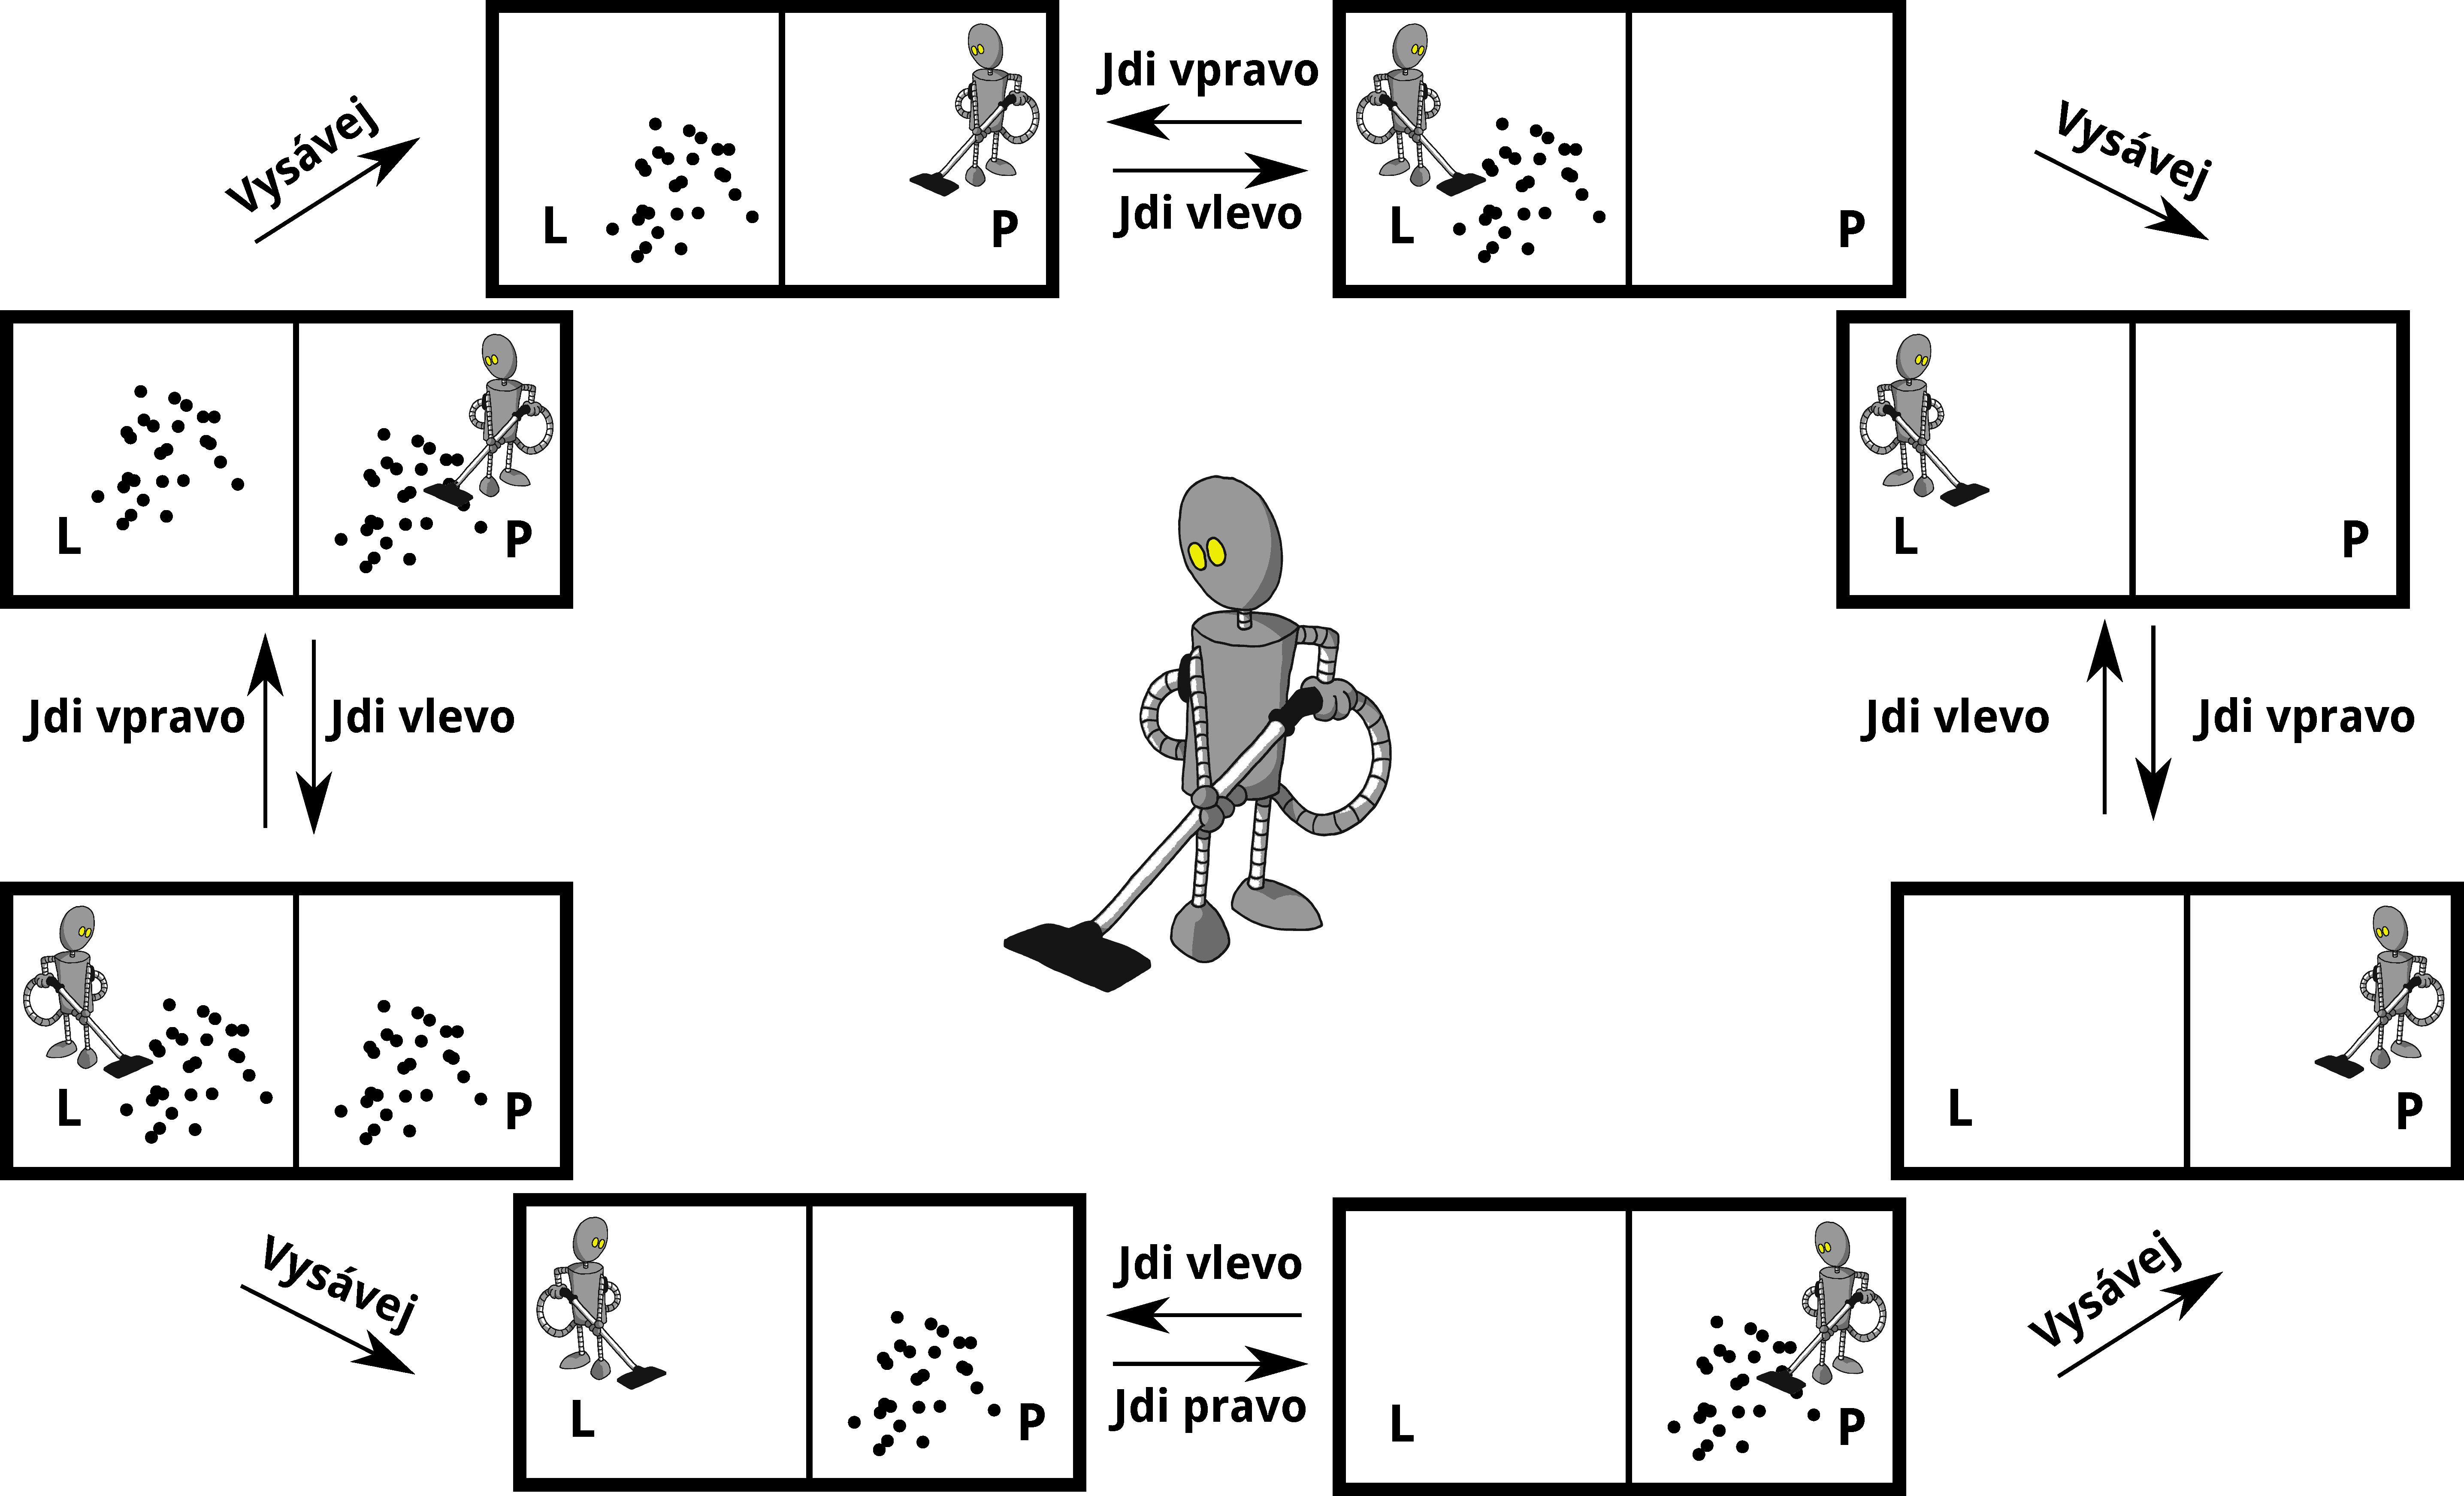
\includegraphics[width=11cm]{vysavaci-graf.pdf}
\end{center} 
\end{frame}

\begin{frame}\frametitle{Agent 008 --- Loydova osmička}
\begin{center}
 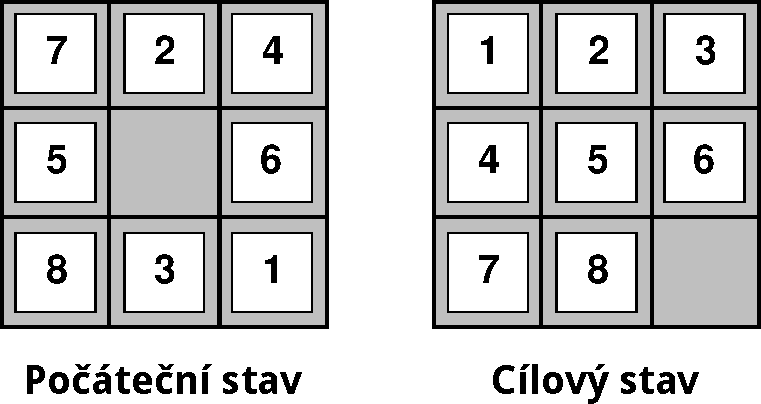
\includegraphics[width=6cm]{loydova-osmicka.pdf}
\end{center}\pause
\begin{itemize}
 \item vrchol grafu \pause --- pozice kostiček \pause
 \item hrana grafu \pause --- pohnutí kostičkou (volným místem)\pause
 \item cílový vrchol \pause --- kostičky jsou srovnané podle čísel\pause
\end{itemize}
\begin{block}{}
 Optimální řešení (t.j. na nejmenší počet tahů) $n$-verze tohoto hlavolamu je NP-těžký problém.
\end{block}

\end{frame}

\begin{frame}\frametitle{Obchodní cestující (TSP)}
\begin{block}{} Obchodní cestující chce navštívit nějaká města a vrátit se na začátek. V jakém pořadí je má navštěvovat tak, aby 
minimalizoval vzdálenost, kterou bude muset urazit?\pause
\end{block}
\begin{itemize}
 \item vrchol grafu \pause --- kombinace následujících údajů: město, ve kterém se obchodní cestující nachází \pause a  stav navštívenosti jednotlivých měst\pause
 \item hrana grafu \pause --- silnice spojující města\pause
 \item cílový vrchol \pause --- vrchol odpovídající počátečnímu město, ve kterém jsou všechna města navštívena
\end{itemize}\pause
NP-těžký problém.
\end{frame}

\begin{frame}\frametitle{Montážní linka}
\begin{center}
 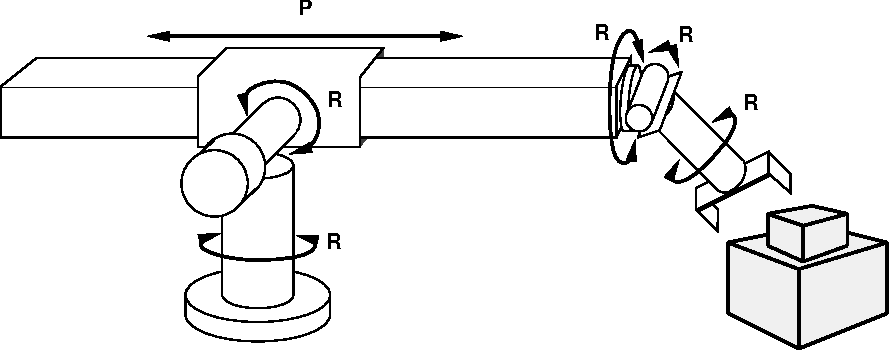
\includegraphics[width=6cm]{montazni-linka.pdf}
\end{center}\pause
\begin{itemize}
 \item vrchol grafu \pause --- kombinace poloh jednotlivých kloubů robotického ramene a jednotlivých součástí\pause
 \item hrana grafu \pause --- pohnutí jednotlivého robotického kloubu\pause
 \item cílový vrchol \pause --- stav, kde jednotlivé součásti jsou složeny
\end{itemize}
\end{frame}

\begin{frame}[fragile]\frametitle{Hledáme řešení --- strom akcí}
\begin{block}{Idea}
Procházet všechny možné posloupnosti akcí a zjistit, která vede k cíli
\end{block}\pause
Postupným procházením vytváříme strom\pause
% \begin{minipage}{5cm}
\begin{itemize}
 \item uzly ve stromu jsou posloupnosti akcí \pause
 \item každému uzlu odpovídá stav světa (po provedení dané posloupnosti akcí)\pause
 \item [] dvěma různým uzlům mohou odpovídat stejné stavy světa (!)\pause
 \item chceme najít uzel, jehož stav je cílovým stavem
\end{itemize}
% \end{minipage}
\end{frame}

\begin{frame}\frametitle{Strom akcí --- robot vysavač}
\begin{center}
\begin{tikzpicture}[node distance=2cm]
\tikzstyle{vertex}=[draw,circle,font={\sffamily\tiny}]
  
% Nulta hladina
\node<1-> [vertex,onslide=<6>{hilight}  ] (koren){l,š,š};
% Prvni hladina
\node<2-> [vertex,below left of  = koren] (lcs1) {l,č,š}; % Vysavej
\node<2-> [vertex,below of       = koren] (pss1) {p,š,š}; % Jdi vpravo
\node<2-> [vertex,below right of = koren,onslide=<6>{hilight}] (lss1) {l,š,š}; % Jdi vlevo
% Druha hladina
% LCS1
\node<3-> [vertex,above left of   = lcs1] (lcs2A) {l,č,š}; % Vysavej
\node<3-> [vertex,left of         = lcs1] (pcs2A) {p,č,š}; % Jdi vpravo
\node<3-> [vertex,below left of   = lcs1] (lcs2A1) {l,č,š}; % Jdi vlevo
% PSS1
\node<4-> [vertex,below left of =  pss1] (psc2B) {p,š,č}; % Vysavej
\node<4-> [vertex,below of =       pss1] (pss2B) {p,š,š}; % Jdi vpravo
\node<4-> [vertex,below right of = pss1,onslide=<6>{hilight}] (lss2B) {l,š,š}; % Jdi vlevo
% LSS1
\node<5-> [vertex,below right of = lss1] (lcs2C) {l,č,š}; % Vysavej
\node<5-> [vertex,right of       = lss1] (pcs2C) {p,š,š}; % Jdi vpravo
\node<5-> [vertex,above right of = lss1] (lcs2C1) {l,š,š}; % Jdi vlevo
\node<6>  [vertex,hilight,below of = lcs2A1] (poznamka) {};
\node<6>  [right of = poznamka] (poznamka2) {\tiny\hskip1cm různé uzly odpovídající stejným stavům};

\path<2->[every node/.style={font=\sffamily\tiny}]
    (koren) edge node [left]  {vysávej} (lcs1)
    (koren) edge node [above] {jdi vpravo} (pss1)
    (koren) edge node [right] {jdi vlevo} (lss1);
\path<3->[every node/.style={font=\sffamily\tiny}]
    (lcs1) edge node [left]  {vysávej} (lcs2A)
    (lcs1) edge node [above] {jdi vpravo} (pcs2A)
    (lcs1) edge node [right] {jdi vlevo} (lcs2A1);
\path<4->[every node/.style={font=\sffamily\tiny}]
    (pss1) edge node [left]  {vysávej} (psc2B)
    (pss1) edge node [above] {jdi vpravo} (pss2B)
    (pss1) edge node [right] {jdi vlevo} (lss2B);
\path<5->[every node/.style={font=\sffamily\tiny}]
    (lss1) edge node [left]  {vysávej} (lcs2C)
    (lss1) edge node [above] {jdi vpravo} (pcs2C)
    (lss1) edge node [right] {jdi vlevo} (lcs2C1);
\end{tikzpicture}
\end{center}
\end{frame}

\begin{frame}\frametitle{Prohledávání stromu akcí--- idea}
\begin{block}{}
 Postupně budujeme strom akcí, dokud nenarazíme na cílový stav.
\end{block}\pause
 \begin{itemize}
  \item v každém kroku dle nějaké strategie vybereme uzel ve stromu akcí\pause
  \item v tomto uzlu strom rozšíříme\pause
  \begin{itemize}
    \item za každou akci, kterou je možné v daném uzlu (resp. stavu) provést
          přidáme do stromu akcí nový uzel
  \end{itemize}
 \end{itemize}
\end{frame}

\begin{frame}[fragile]\frametitle{Prohledávání stromů --- tree search}
\begin{python}
def treeSearch( problem, strategy ):
    # Inicializuj strom.
    tree = node(problem.initial_state())
    while True:
      # Zvol kandidata k expanzi dle strategie.
      leaf_node = strategy(problem, tree)
      # Mame reseni,vrat posloupnost kroku.
      if problem.is_goal( leaf_node.state() ):
        return leaf_node
      # Expanduj kandidata (pridej do stromu 
      # uzly, ktere sousedi s kandidatem).
      stav = leaf_node.state()
      for a in stav.possible_actions():
        nb_stav = stav.act(a)
        leaf_node.add_child( a, node(nb_stav) )
\end{python}
\end{frame}

\begin{frame}\frametitle{Prohledávací strategie --- hodnotící kritéria}
% \begin{block}{}
% Strategii definujeme tak, že určíme pořadí, v jakém budeme expandovat uzly
% \end{block}

\begin{itemize}
 \item úplnost\pause\ (vždy nalezne cílový stav, pokud existuje)\pause
 \item optimálnost\pause\ (posloupnost akcí vedoucí do cílového stavu bude optimální)\pause
 \item časová složitost\pause\ (kolik uzlů je třeba vygenerovat)\pause
 \item paměťová náročnost\pause\ (kolik uzlů je třeba držet v paměti)\pause
\end{itemize}

Časová složitost a paměťová náročnost se měří jako funkce\pause
\begin{itemize}
 \item[b] --- faktor větvení (branching factor)\pause
 \item[d] --- hloubka optimálního řešení\pause
 \item[m] --- hloubka prohledávaného stromu
\end{itemize}

\end{frame}


\begin{frame}\frametitle{Prohledávací strategie --- uninformed search}
% Příště: informed search, heuristiky
\begin{itemize}
 \item prohledávání do šířky (BFS)\pause
 \item prohledávání do hloubky (DFS)\pause
 \item omezená hloubka (depth limited, DLS)\pause
 \item iterování hloubky (iterative deepening, IDS)\pause
\end{itemize}
\end{frame}


\begin{frame}[fragile]\frametitle{BFS --- prohledávání do šířky}
\begin{tikzpicture}[grow=right]
\tikzstyle{level 1}=[level distance=1.5cm, sibling distance=3.5cm]
\tikzstyle{level 2}=[level distance=1.5cm, sibling distance=2cm]
\tikzstyle{level 3}=[level distance=1.5cm, sibling distance=1cm]
\tikzstyle{vertex}=[draw,circle,font={\sffamily\tiny}]
\node[vertex,onslide=<3|handout:3>{active},onslide=<2|handout:2>{memory}] {0}
 child {node[vertex,onslide=<4-5|handout:4-5>{active},onslide=<3|handout:3>{memory}] {00}
         child {node (000)[vertex,onslide=<8-9|handout:8-9>{active},onslide=<5-7|handout:5-7>{memory}] {000} 
                 child { node[vertex,onslide=<16|handout:16>{active},onslide=<9-15|handout:9-15>{memory}] {0000} }
                 child { node[vertex,onslide=<17|handout:17>{active},onslide=<9-16|handout:9-16>{memory}] {0001} }
               }
         child {node (001)[vertex,onslide=<10-11|handout:10-11>{active},onslide=<5-9|handout:5-9>{memory}] {001} 
                 child { node[vertex,onslide=<18|handout:18>{active},onslide=<11-17|handout:11-17>{memory}] {0010} }
                 child { node[vertex,onslide=<19|handout:19>{active},onslide=<11-18|handout:11-18>{memory}] {0011} }
               }               
       }
 child {node[vertex,onslide=<6-7|handout:6-7>{active},onslide=<3-5|handout:3-5>{memory}] {01}
         child {node (010)[vertex,onslide=<12-13|handout:12-13>{active},onslide=<7-11|handout:7-11>{memory}] {010}
                 child { node[vertex,onslide=<20|handout:20>{active},onslide=<13-19|handout:13-19>{memory}] {0100} }
                 child { node[vertex,onslide=<21|handout:21>{active},onslide=<13-20|handout:13-20>{memory}] {0101} }
               }
         child {node (011)[vertex,onslide=<14-15|handout:14-15>{active},onslide=<7-13|handout:7-13>{memory}] {011}
                 child { node[vertex,onslide=<22|handout:22>{active},onslide=<15-21|handout:15-21>{memory}](0110) {0110} }
                 child { node[vertex,onslide=<23|handout:23>{active},onslide=<15-22|handout:15-22>{memory}](0111) {0111} }
               }               
       };
\node<1->  [vertex,active,right of = 0111] (poznamkaA) {};
\node<1->  [right=0.2cm of poznamkaA] (poznamkaA2) {\begin{minipage}{4cm}\tiny uzel zvolený k expanzi\end{minipage}};
\node<1->  [vertex,memory,right of = 0110] (poznamkaM) {};
\node<1->  [right=0.2cm of poznamkaM] (poznamkaM2) {\begin{minipage}{4cm}\tiny potenciální kandidát k expanzi\\ (nutno udržovat v paměti)\end{minipage}};
\end{tikzpicture}
\end{frame}

\begin{frame}\frametitle{BFS --- prohledávání do šířky}
 \begin{itemize}
  \item úplnost:\pause\ ANO (pokud je $b$ konečné)\pause
  \item časová složitost:\pause\ $1$\pause\ $+\ b$\pause\ $+\ b^2$\pause\ $ +\cdots+ b(b^d - 1)$\pause\ $= O(b^{d+1})$\pause
  \item \alert<14>{paměťová náročnost}:\pause\ $O(b^{d+1})$ (celý strom akcí se uchovává v paměti)\pause
  \item optimalita:\pause\ to závisí\pause\ (ano, pokud všechny akce stojí stejně, jinak je třeba modifikovat)
 \end{itemize}\pause
 
 \begin{center}
Největším problémem je paměťová náročnost.
 \end{center}\pause
 \begin{center}
 b = 10, 10000 uzlů/sec., uzel = 1Kb
 \begin{tabular}{cccc}
 {\bf hloubka} 	& {\bf uzly} 	& {\bf čas } 	& {\bf paměť}\cr
 \hline
 2		& 1100		& 0.1 s 	&  1 Mb\cr
 4		& 111100	& 11 s 		&  106 Mb\cr
 6		& $10^7$	& 19 min 	&  10 Gb\cr
 8		& $10^9$	& 31 h 		&  \alert{1 Tb}\cr
 10		& $10^{11}$	& 129 dní	&  101 Tb\cr
 12		& $10^{13}$	& \alert{35 let}&  10 Petabyte\cr
 14		& $10^{15}$	& 3523 let	&  1 Exabyte\cr
 \hline
 \end{tabular}
 \end{center}
\end{frame}

\begin{frame}\frametitle{DFS --- prohledávání do hloubky}
\begin{tikzpicture}[grow=right]
\tikzstyle{level 1}=[level distance=1.5cm, sibling distance=3.5cm]
\tikzstyle{level 2}=[level distance=1.5cm, sibling distance=2cm]
\tikzstyle{level 3}=[level distance=1.5cm, sibling distance=1cm]
\tikzstyle{vertex}=[draw,circle,font={\sffamily\tiny}]
\node[vertex,onslide=<3|handout:3>{active},onslide=<2|handout:2>{memory}] {0}
 child {node[vertex,onslide=<4-5|handout:4-5>{active},onslide=<3|handout:3>{memory}] {00}
         child {node (000)[vertex,onslide=<6-7|handout:6-7>{active},onslide=<5|handout:5>{memory}] {000} 
                 child { node[vertex,onslide=<8|handout:8>{active},onslide=<7|handout:7>{memory}] {0000} }
                 child { node[vertex,onslide=<9|handout:9>{active},onslide=<7-8|handout:7-8>{memory}] {0001} }
               }
         child {node (001)[vertex,onslide=<10-11|handout:10-11>{active},onslide=<5-9|handout:5-9>{memory}] {001} 
                 child { node[vertex,onslide=<12|handout:12>{active},onslide=<11|handout:11>{memory}] {0010} }
                 child { node[vertex,onslide=<13|handout:13>{active},onslide=<11-12|handout:11-12>{memory}] {0011} }
               }               
       }
 child {node[vertex,onslide=<14-15|handout:14-15>{active}] {01}
         child {node (010)[vertex,onslide=<16-17|handout:16-17>{active},onslide=<15|handout:15>{memory}] {010}
                 child { node[vertex,onslide=<18|handout:18>{active},onslide=<17|handout:17>{memory}] {0100} }
                 child { node[vertex,onslide=<19|handout:19>{active},onslide=<17-18|handout:17-18>{memory}] {0101} }
               }
         child {node (011)[vertex,onslide=<20-21|handout:20-21>{active},onslide=<15-19|handout:15-19>{memory}] {011}
                 child { node[vertex,onslide=<22|handout:22>{active},onslide=<21|handout:21>{memory}](0110) {0110} }
                 child { node[vertex,onslide=<23|handout:23>{active},onslide=<21-22|handout:21-22>{memory}](0111) {0111} }
               }               
       };
\node<1->  [vertex,active,right of = 0111] (poznamkaA) {};
\node<1->  [right=0.2cm of poznamkaA] (poznamkaA2) {\begin{minipage}{4cm}\tiny uzel zvolený k expanzi\end{minipage}};
\node<1->  [vertex,memory,right of = 0110] (poznamkaM) {};
\node<1->  [right=0.2cm of poznamkaM] (poznamkaM2) {\begin{minipage}{4cm}\tiny potenciální kandidát k expanzi\\ (nutno udržovat v paměti)\end{minipage}};       
       
% \node[vertex,onslide=<2-3>{active},onslide=<4->{memory}] {0}
%  child {node[vertex,onslide=<4-5>{active},onslide=<3>{memory},onslide=<6-13>{memory}] {00}
%          child {node (000)[vertex,onslide=<6-7>{active},onslide=<5>{memory},onslide=<8-9>{memory}] {000} 
%                  child { node[vertex,onslide=<8>{active},onslide=<7>{memory}] {0000} }
%                  child { node[vertex,onslide=<9>{active},onslide=<7-8>{memory}] {0001} }
%                }
%          child {node (001)[vertex,onslide=<10-11>{active},onslide=<5-9>{memory},onslide=<12-13>{memory}] {001} 
%                  child { node[vertex,onslide=<12>{active},onslide=<11>{memory}] {0010} }
%                  child { node[vertex,onslide=<13>{active},onslide=<11-12>{memory}] {0011} }
%                }               
%        }
%  child {node[vertex,onslide=<14-15>{active},onslide=<16->{memory}] {01}
%          child {node (010)[vertex,onslide=<16-17>{active},onslide=<15>{memory},onslide=<18-19>{memory}] {010}
%                  child { node[vertex,onslide=<18>{active},onslide=<17>{memory}] {0100} }
%                  child { node[vertex,onslide=<19>{active},onslide=<17-18>{memory}] {0101} }
%                }
%          child {node (011)[vertex,onslide=<20-21>{active},onslide=<15-19>{memory},onslide=<22->{memory}] {011}
%                  child { node[vertex,onslide=<22>{active},onslide=<21>{memory}] {0110} }
%                  child { node[vertex,onslide=<23>{active},onslide=<21-22>{memory}] {0111} }
%                }               
%        };       
\end{tikzpicture}

\end{frame}

\begin{frame}\frametitle{DFS --- prohledávání do hloubky}
\begin{itemize}
  \item úplnost:\pause\ NE (pokud je hloubka nekonečná\pause\ nebo pokud jsou smyčky)\pause
  \item časová složitost:\pause\ $O(b^m)$\pause
  \begin{itemize}
  \item problém, pokud je $d<<m$
  \item pokud jsou řešení hustě rozložená, je mnohem rychlejší než BFS
  \end{itemize}
  \item paměťová náročnost:\pause\ $O(m)$ (\alert{lineární}!)\pause
  \item optimalita:\pause\ NE
 \end{itemize}\pause
\end{frame}

\begin{frame}\frametitle{DLS,IDS --- prohledávání do omezené hloubky}
\begin{itemize}
\item[DLS] --- prohledávání do hloubky, ale strom usekneme na hladině $l$ a hlouběji
nejdeme.\pause
\item[IDS] --- postupně aplikujeme DLS s větším a větším $l$\pause
\end{itemize}
\begin{itemize}
  \item úplnost:\pause\ ANO\pause
  \item časová složitost:\pause\ $O(b^d)$\pause
  \item paměťová náročnost:\pause\ $O(d)$ (\alert{lineární}!)\pause
  \item optimalita:\pause\ ANO (pokud všechny akce stojí stejně, jinak je třeba modifikovat)
 \end{itemize}\pause
\end{frame}


\begin{frame}\frametitle{Prohledávání z obou konců}
\end{frame}

\begin{frame}\frametitle{Částečně pozorovatelné, nedeterminované světy}
\end{frame}

\end{document}


